% =====================================================================
%  SFTF -- main manuscript for 3D Printing and Additive Manufacturing (TDP), SAGE
%  Article type: Original Article
%    limits: 4000 words body | abstract <300w | <=8 figures | <=5 tables | <=100 refs
%  Restructured from the PiAM draft (SFTF_draft.tex) into TDP IMRaD form:
%    Introduction / Materials and Methods / Results / Discussion / Conclusions.
%  Table budget: 5 tables kept here; 6 moved to the Supplement (S7-S12).
%    See SFTF_TDP_supplementary.tex.
%  Review type: single-anonymized -> author identity NOT hidden (self-citation & repo link OK).
%  Reference style: Sage Vancouver (numeric). Swap unsrtnat for the official
%    SAGE Vancouver .bst at submission.
% =====================================================================
% !TEX program = pdflatex
\documentclass[12pt]{article}

\usepackage[utf8]{inputenc}
\usepackage[T1]{fontenc}
\usepackage{amsmath,amssymb,amsthm,bm}
\usepackage{graphicx}
\usepackage[labelfont=bf,labelsep=space]{caption}
\captionsetup[figure]{name=Fig.}
\usepackage{booktabs}
\usepackage{float}
\usepackage[numbers,sort&compress]{natbib}
\usepackage{setspace}
\usepackage[margin=25mm]{geometry}
\usepackage{lineno}
\usepackage{xcolor}
\usepackage[hidelinks]{hyperref}
\usepackage{fancyhdr}

\doublespacing            % TDP: double-spaced manuscript
\linenumbers

% running head (<= 50 chars incl. spaces)
\pagestyle{fancy}\fancyhf{}
\fancyhead[R]{\small SFTF for Build-Orientation Candidate Generation}
\fancyfoot[C]{\thepage}
\renewcommand{\headrulewidth}{0.4pt}

% --- drafting convenience: placeholder if a figure asset is missing ---------
% (keeps the file compiling with or without the pics/ folder; harmless at submit)
\let\origincludegraphics\includegraphics
\renewcommand{\includegraphics}[2][]{%
  \IfFileExists{#2}{\origincludegraphics[#1]{#2}}%
  {\fbox{\parbox[c][2.5cm][c]{0.75\linewidth}{\centering\ttfamily\small [missing figure asset]}}}}

\newtheorem{definition}{Definition}
\newtheorem{theorem}{Theorem}
\newtheorem{proposition}{Proposition}

\title{Support Flow Tensor Field for Fast Build-Orientation Candidate Generation
in Support-Requiring Additive Manufacturing}
\author{InHwan Sul\\
\small Department of Materials Design Engineering, Kumoh National Institute of Technology,\\
\small Gumi 39177, Republic of Korea\\
\small Email: snowman0@kumoh.ac.kr \quad ORCID: 0000-0003-0105-920X}
\date{}
\newcommand{\TODO}[1]{\textcolor{red}{[\textbf{TODO}: #1]}}

\begin{document}
\maketitle

% ============================ ABSTRACT ( <300 words ) =================
\begin{abstract}
\noindent
Build orientation strongly controls support volume in additive manufacturing, but
exhaustive orientation sweeps remain costly. The proposed method targets
support-requiring processes in which build orientation changes the amount of
removable support material; it is not intended for inherently support-free
processes. This paper proposes the Support Flow Tensor Field (SFTF), a fast
candidate generator that ranks promising build directions before local
verification by a support-volume grid or slicer. For each sampled direction, SFTF
casts rays from overhang faces to actual receiver faces and forms a
direction-dependent asymmetric flow tensor; the build-plate support term is
interpreted as a virtual ground receiver, making the dominant predictive term a
unified Rayleigh cost. On five organic freeform benchmark meshes with a $1^\circ$
tomography grid, verifying the $\pm 10^\circ$ neighborhoods of the top-$20$ SFTF
candidates uses $3.40\%$ of the grid on average and obtains a mean support-volume
ratio of $1.14$ (maximum $1.66$); the tensor features $B$ and $\tilde R=R+B$ are the
most stable single predictors of the tomographic support volume (mean Spearman
$0.59$ and $0.61$). We also introduce Adaptive Verification Escalation (AVE), an
automatic hard-case escalation rule based on local-verification confidence signals;
on a five-group cached $1^\circ$ audit of $21$ ratio-valid records it keeps every
record below ratio $2.0$ (mean $1.14$, maximum $1.93$) at a mean budget of
$13.94\%$. We report a clear limitation: on large mechanical parts (up to $1.04$M
faces) the tensor features do not predict support volume, and at a matched budget a
simple uniform-axis window seeding outperforms the SFTF ranking. SFTF is therefore
best positioned as an interpretable warm start for organic parts that concentrates
expensive verification on a small number of likely basins rather than replacing
broad coverage.
\end{abstract}

\noindent\textbf{Keywords:} Support Flow Tensor Field (SFTF); build orientation;
support volume; support-requiring additive manufacturing; local verification;
candidate generation

% ============================ 1. INTRODUCTION ========================
\section{Introduction}

Build orientation strongly affects support volume, material use, print time, and
post-processing quality in support-requiring additive manufacturing, especially FDM
processes in which downward overhangs beyond a critical angle require removable
support~\cite{gibson}. Existing explicit or voxel/slicer-based orientation searches
can evaluate support volume accurately, but exhaustive yaw--pitch sweeps remain
expensive because they evaluate a dense set of directions even for simple shapes.

\subsection{Related work}
\label{sec:related}
Build-orientation studies include explicit support-volume evaluation, voxel/depth-normal
acceleration, support-structure design, and topology or multi-axis design
approaches~\cite{das2017,wang2010,vaissier2019,jiang2018,mirzendehdel2016,langelaar2018,dai2018}.
Shadow-volume and tomographic formulations estimate support volume without full
slicer generation and can also be accelerated on GPUs~\cite{ezair,msst,gpumsst}. In
this manuscript, TOMO\_CPU and TOMO\_CUDA denote the CPU and GPU tomographic
support-volume evaluators used as verification and comparison backends~\cite{gpumsst};
SFTF is instead a candidate generator that reduces the number of directions passed
to such verifiers. Tensor or anisotropic formulations have also appeared in topology
optimization, where overhang constraints, anisotropic interface energy, and
deposition-direction-dependent stiffness bias a redesigned part toward
self-supporting geometry~\cite{gaynor2014,garcke2023,shin2025}. The present work is
complementary: the input shape is fixed, and the tensor is used only to rank build
orientations before an accurate TOMO or slicer verification step. A related
industrial patent seeks build orientations for fixed complex parts but does not
disclose an open algorithmic procedure~\cite{smith2025patent}.

\subsection{Contribution}
This paper proposes the Support Flow Tensor Field (SFTF), a low-cost candidate
generator rather than a replacement for precise TOMO/slicer optimization. For each
sampled build direction, SFTF estimates internal face-to-face support flow by ray
casting, adds a build-plate contribution through a virtual ground node, and passes
only a small set of promising basins to local TOMO verification. The main
contributions are: (i) a direction-dependent asymmetric support-flow tensor for
fixed parts; (ii) a ground-node derivation showing that the build-plate term is an
exact Rayleigh contribution of the augmented tensor; (iii) a local-verification
budget curve demonstrating that on organic freeform meshes SFTF top-$20$ windows
recover a mean support-volume ratio of $1.14$ with only $3.40\%$ of the $1^\circ$
grid; (iv) Adaptive Verification Escalation (AVE), an automatic escalation rule for
narrow-basin hard cases; (v) a five-group timing audit showing $8.3$--$381.9\times$
Python and $56.8$--$56{,}027\times$ C++ speedups relative to TOMO\_CPU on the same
$1^\circ$ sweep; and (vi) an honest characterization of where the method breaks
down---on large mechanical parts the tensor features stop predicting support volume
and a budget-matched uniform-axis control outperforms the ranking (\S\ref{sec:limits}).

% ============================ 2. MATERIALS AND METHODS ===============
\section{Materials and Methods}

\subsection{From symmetric support tensor to directional flow}
\label{sec:sftf}
As a symmetric baseline, we define an area-weighted second-moment tensor of face
normals
\begin{equation}
M=\sum_i A_i m_i m_i^T,
\end{equation}
following the general orientation/fabric-tensor construction for directional
data~\cite{kanatani1984}. Here $A_i$ and $m_i$ are the area and outward normal of
triangular face $i$. This tensor summarizes the distribution of surface normals but
does not encode whether a face is an overhang for a given build direction, whether
another face can receive the support, or how far an unsupported face is from the
build plate. SFTF therefore evaluates a direction-dependent asymmetric tensor for
each unit build direction $n\in S^2$. For face centroid $c_i$, the overhang
coefficient is
\begin{equation}
O_i(n)=\max(0,-m_i\cdot n).
\end{equation}
For sampled overhang source faces, a ray is cast along $-n$; if the first valid
receiver is face $j$, the height is $h_{ij}(n)=(c_i-c_j)\cdot n$ and the face-to-face
influence is
\begin{equation}
w_{ij}(n)=\frac{O_i(n)}{1+\alpha h_{ij}(n)}, \qquad \alpha=1/D,
\end{equation}
where $D$ is the mesh bounding-box diagonal. The face-to-face support flow tensor is
\begin{equation}
F(n)=\sum_{(i,j)\in\mathcal{R}(n)} w_{ij}(n)A_iA_jm_im_j^T,
\label{eq:sftf-tensor}
\end{equation}
with $\mathcal{R}(n)$ the valid ray-cast support relationships. The receiver must not
be the source face, must have positive height, and must face the build direction
sufficiently ($m_j\cdot n>0.05$). To bound cost, source faces are sampled
deterministically in proportion to $A_iO_i(n)$ using
\begin{equation}
K_{ray}=\mathrm{clip}(0.02N_f,500,3000),
\label{eq:kray-budget}
\end{equation}
where $N_f$ is the number of mesh faces. When the number of positive-weight source
faces exceeds $K_{ray}$, the quantity computed is the plug-in estimator of
Eq.~\eqref{eq:sftf-tensor} restricted to the sampled source set $\mathcal{S}(n)$,
\begin{equation}
\hat F(n)=\sum_{\substack{(i,j)\in\mathcal{R}(n)\\ i\in\mathcal{S}(n)}} w_{ij}(n)A_iA_jm_im_j^T,
\label{eq:sftf-tensor-estimator}
\end{equation}
where $\mathcal{S}(n)$ is selected by deterministic systematic sampling on the
cumulative weight $A_iO_i(n)$ (fixed half-interval offsets, no random seed); the
scalar features $R$, $P$, and $B$ inherit the same restriction, and the sum is exact
whenever the positive-weight sources number at most $K_{ray}$. No inverse-probability
reweighting is applied, so $\hat F$ is a deterministic budget-normalized surrogate
used only to compare directions of the same mesh under an identical budget and
sampling rule.

\subsection{Ground-node build-plate term}
\label{sec:groundnode}
If no valid receiver face is found, the overhang is ultimately supported from the
build plate. With
\begin{equation}
z_{plate}(n)=\min_{v\in V}v\cdot n,\qquad h_{iP}(n)=c_i\cdot n-z_{plate}(n),
\end{equation}
the scalar plate penalty is
\begin{equation}
B(n)=\sum_{i\in\mathcal{B}(n)}O_i(n)A_i(1+\alpha h_{iP}(n)).
\end{equation}
As illustrated in Fig.~\ref{fig:unified-flow}, this term is exactly the Rayleigh
contribution obtained by adding a virtual receiver whose normal is the build
direction $n$,
\begin{equation}
\tilde F(n)=\sum_{(i,j)\in\mathcal{R}(n)} w_{ij}(n)A_iA_jm_im_j^T+
\sum_{i\in\mathcal{B}(n)} A_i(1+\alpha h_{iP})m_in^T.
\end{equation}
Since $m_i\cdot n=-O_i(n)$, the symmetric Rayleigh contraction of the ground term
contributes exactly $B(n)$ to the support cost, giving
\begin{equation}
\tilde R(n)=\max(0,-n^T\tilde F_s(n)n)=R(n)+B(n).
\label{eq:Rtilde}
\end{equation}
The equality was numerically confirmed within $10^{-12}$ over the stored candidate pools.

\begin{figure}[H]
\centering
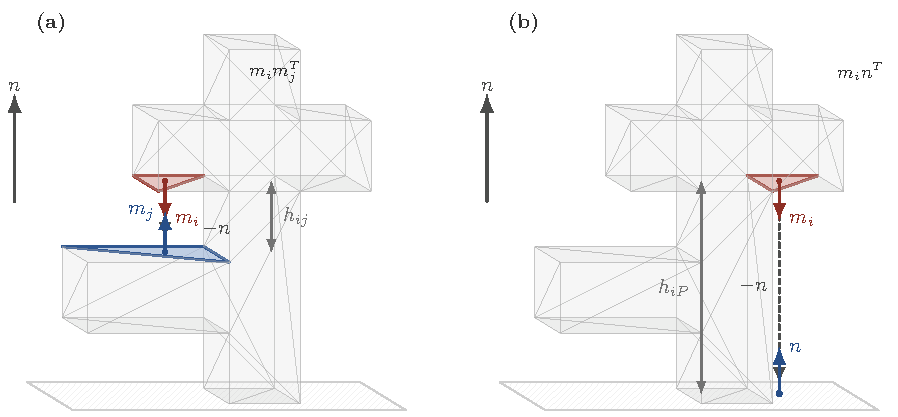
\includegraphics[width=0.9\textwidth]{pics/FTree4x_fig1_unified_flow.pdf}
\caption{Unified flow interpretation. Face-to-face support uses receiver normal
$m_j$, while direct build-plate support is represented by a virtual receiver with
normal $n$; the latter gives the Rayleigh contribution $B(n)$ in Eq.~\eqref{eq:Rtilde}.}
\label{fig:unified-flow}
\end{figure}

\subsection{Candidate generation and rescoring}
The deployed score is
\begin{equation}
J(n)=\tilde R(n)+P(n),\qquad
P(n)=\sum_{(i,j)\in\mathcal{R}(n)}O_i(n)A_iA_j,
\end{equation}
where $P$ is the face-to-face overhang amount after the height attenuation in
$w_{ij}$ cancels. Because $O_i$, $w_{ij}$, and $\alpha h$ are dimensionless, $R$ and
$P$ carry units of area squared while $B$ carries units of area: under a uniform
rescaling by $s$, $R$ and $P$ scale as $s^4$ whereas $B$ scales as $s^2$, so
$J=\tilde R+P=R+P+B$ is unit-dependent and is treated as a screening feature only. A
$512$-direction Fibonacci-sphere sample is first evaluated, the best directions are
locally resampled in $2^\circ$--$8^\circ$ cones, and angular non-maximum suppression
keeps separated candidates. To avoid treating dimensionally different quantities as
commensurate, the final candidate order uses rank-normalized
features\footnote{Rank tuning denotes fitting weights after converting each feature
to its within-candidate rank; it is an empirical candidate-ranking calibration, not
continuous geometric optimization.} $[J,R,P,B,H,S,\sigma_1]$, following the standard
rank-transformation idea for scale-robust empirical modeling~\cite{conover1981rank};
the rank transform makes the final ordering invariant to any strictly monotone
rescaling of each feature. Here $H$ is the valid-hit count and $S,\sigma_1$ are
singular-value features retained only for post-processing. The reported calibration
uses weights $(w_J,w_R,w_P,w_B,w_H,w_S,w_1)=(0,0.731,-2.3897,2.1447,2.3109,-2.2922,1.6363)$.
Implementation optimizations, including first-hit fallback and per-mesh cached
geometry, reduced a 1k-direction evaluation of \emph{Bunny 69k} from about $15.7$~s
to $1.5$~s without changing selected directions.

\subsection{Datasets and experimental environment}
\label{sec:datasets}
The dataset consists of five groups that deliberately separate \emph{shape
difficulty} from \emph{mesh scale}. Groups A--C set the scale in the
$\sim$$10^1$--$10^5$-face range and vary difficulty from basic to freeform organic
shapes, revealing the \emph{fixed-cost floor} of the exhaustive sweep; groups D--E
fix the difficulty as real manufacturing parts while pushing the scale from $256$ to
$1.04\times10^6$ faces, revealing the \emph{adaptive cost} of SFTF candidate
evaluation. Group~A: basic shapes (cube, sphere, cylinder, cone, torus, $\sim$$10^1$--$10^3$
faces). Group~B: simple functional parts (u\_bracket, hook, c\_clamp, pipe\_elbow,
hollow\_box). Group~C: organic/freeform benchmarks (\emph{Bunny 69k}, \emph{Manikin
13k}, \emph{Dragon 100k}, \emph{Happy 50k}, \emph{Lucy 50k}). Group~D: Thingi10K set~1,
$256$--$88{,}106$ faces~\cite{Thingi10K}. Group~E: Thingi10K set~2, about
$5.1\times10^5$--$1.04\times10^6$ faces. All timing used a Windows~11 workstation with
an AMD Ryzen~9 9950X3D CPU (16 cores/32 threads), 125~GB RAM, and an NVIDIA GeForce
RTX~5080 GPU (16~GB). The Python implementation used Python~3.12 with NumPy, SciPy,
Trimesh, and scikit-learn; TOMO\_CPU/TOMO\_CUDA were called through Windows DLL
interfaces, and SFTF\_C++ was built as an x64 C++ DLL (MSVC, OpenMP).

\subsection{Comparison targets and evaluation protocol}
\label{sec:protocol}
The comparison targets are: (1) PCA-based direction; (2) existing Support Tensor
eigenvector direction; (3) initial eigenvector-based concave direction; (4) this
study's SFTF direction; and (5) TOMO\_CPU or commercial-slicer-based $v_{ss}$ optimal
direction. For each mesh we generate a $v_{ss}$ contour at $1^\circ$ intervals under a
critical angle of $60^\circ$, and evaluate how close the $v_{ss}$ value at our top
candidate directions is to the global optimum; if the $v_{ss}$ values are similar we
regard directions as optimal orientations of the same level. Because the global
optimum can be scattered across multiple basins, we compare angularly separated
top-$k$ basin representatives, re-inputting SFTF candidate basins to TOMO\_CPU to
measure $M_{ss}$ directly. Unless otherwise stated, both the five-mesh accuracy
results and the A--E audit use stored $1^\circ$ TOMO\_CPU grids. Ratio statistics at
$\theta_c=60^\circ$ exclude records whose TOMO global best is nonpositive, because
those cases make a positive support-volume ratio ill-defined.

% ============================ 3. RESULTS =============================
\section{Results}

\subsection{Stored TOMO grid comparison}
The stored $1^\circ$, $\theta_c=60^\circ$ TOMO\_CPU grids were used as the accuracy
reference. SFTF candidates were mapped to the nearest signed TOMO yaw--pitch cell,
and ratios were computed against the global TOMO best value
(Table~\ref{tab:sftf-tomo-comparison}). Raw ranking alone is insufficient for the
\emph{Happy 50k} hard case (ratio $2.34$), so SFTF is used as a warm start for local
TOMO verification rather than as a standalone optimizer.

\begin{table}[H]
\centering
\caption{Stored TOMO\_CPU $v_{ss}$ grid versus the current SFTF candidates. Ratio is
the SFTF candidate's $v_{ss}$ over the TOMO global optimum.}
\label{tab:sftf-tomo-comparison}
\begin{tabular}{lrrrrr}
\toprule
Mesh & TOMO best & SFTF score1 & Ratio & SFTF best-of-3 & Ratio\\
\midrule
\emph{Bunny 69k} & 4440.34 & 5217.86 & 1.18 & 5217.86 & 1.18\\
\emph{Manikin 13k} & 2956.12 & 5565.56 & 1.88 & 5565.56 & 1.88\\
\emph{Dragon 100k} & 28106.97 & 37640.00 & 1.34 & 36067.25 & 1.28\\
\emph{Happy 50k} & 8512.64 & 19894.23 & 2.34 & 18592.73 & 2.18\\
\emph{Lucy 50k} & 7605.40 & 9132.08 & 1.20 & 9132.08 & 1.20\\
\bottomrule
\end{tabular}
\end{table}

\subsection{Local verification and adaptive verification escalation}
\label{sec:ave}
The deployed metric is a budget curve: the top-$K$ SFTF candidates define
$\pm10^\circ$ local windows, and the best TOMO grid value inside their union is
selected (Table~\ref{tab:budget-curve}). At top-$20$, the mean support-volume ratio
is $1.14$ (maximum $1.66$) using only $3.40\%$ of the $1^\circ$ grid. A budget-matched
farthest-point uniform-axis control performs on par with SFTF on these organic meshes
and is slightly better in the worst case (Supplementary Table~S7), so on organic parts
the warm-start value is the small verified budget rather than the exact window
placement; \S\ref{sec:limits} shows the two diverge sharply on large parts.

\begin{table}[H]
\centering
\caption{Budget curve of top-$K$ local TOMO verification around SFTF candidates. The
budget is the mean fraction of the $1^\circ$ TOMO grid covered by the union of local
windows.}
\label{tab:budget-curve}
\begin{tabular}{rrrrrr}
\toprule
Top-$K$ & Mean ratio & Median ratio & Max ratio & Mean grid budget & Ratio $\le 2.0$\\
\midrule
3  & 1.24 & 1.07 & 1.97 & 0.87\% & 5/5\\
10 & 1.18 & 1.02 & 1.84 & 2.03\% & 5/5\\
20 & \textbf{1.14} & \textbf{1.00} & \textbf{1.66} & 3.40\% & 5/5\\
30 & 1.14 & 1.00 & 1.66 & 5.20\% & 5/5\\
\bottomrule
\end{tabular}
\end{table}

Adaptive Verification Escalation (AVE) escalates only when ordinary top-$10$ local
verification is uncertain (organic-mesh result in Supplementary Table~S8). The trigger
uses local-verification quantities only,
\begin{equation}
\begin{aligned}
\mathrm{trigger}_{\mathrm{AVE}}
&=[\eta\ge0.008]\wedge[\mathrm{edge}=1\vee g\le1.5\vee g\ge3.0],\\
\eta&=V_{ss}^{\mathrm{loc}}/V_{\mathrm{bbox}},\qquad
 g=V_{ss}^{\mathrm{seed}}/V_{ss}^{\mathrm{loc}},
\end{aligned}
\label{eq:ave-trigger}
\end{equation}
where $\mathrm{edge}=1$ means the best local cell lies within $1^\circ$ of a window
boundary, a small gain $g\le1.5$ means the window search barely improved on the seed
(a plateau), and a large gain $g\ge3.0$ means it moved far (an unreliable seed).
Escalation only expands the verified candidate set, so it can spend more budget but
cannot worsen the selected value. Table~\ref{tab:ave-g5} reports the held-out cached
A--E audit of $21$ ratio-valid records (after excluding $14$ with nonpositive TOMO
best at $\theta_c=60^\circ$). The valid set is larger than in the original submission
because a $16$-bit per-column overflow in the TOMO\_CPU voxel accumulator had
corrupted the support volume of the high-face-count group-E meshes; with the
accumulator corrected, those meshes yield positive optima and become ratio-valid.

\begin{table}[H]
\centering
\caption{Cached five-group audit of the tiered AVE policy on ratio-valid $1^\circ$,
$\theta_c=60^\circ$ TOMO\_CPU records. The top-$10$ baseline over all ratio-valid
records has mean ratio $5.10$, maximum $62.59$, mean budget $2.26\%$, and $14/21$
below ratio $2.0$.}
\label{tab:ave-g5}
\small
\begin{tabular}{lrrrrrr}
\toprule
Group & $n$ & Expanded & Mean & Max & Budget & $\le 2.0$\\
\midrule
A & 2 & 2 & 1.03 & 1.06 & 7.59\% & 2/2\\
B & 1 & 1 & 1.10 & 1.10 & 6.97\% & 1/1\\
C & 5 & 3 & 1.14 & 1.66 & 9.99\% & 5/5\\
D & 6 & 5 & 1.03 & 1.13 & 23.58\% & 6/6\\
E & 7 & 7 & 1.26 & 1.93 & 11.30\% & 7/7\\
\midrule
All & 21 & 18 & \textbf{1.14} & \textbf{1.93} & \textbf{13.94\%} & 21/21\\
\bottomrule
\end{tabular}
\end{table}

The audit reduces the maximum ratio from $62.59$ to $1.93$ and keeps all ratio-valid
records below $2.0$ at a mean budget of $13.94\%$ (under one seventh of the $1^\circ$
grid). The single hardest case is the $1.04$M-face \emph{Group\_E2\_790253} at ratio
$1.93$, marking the practical ceiling of coarse SFTF coverage on large parts.
Representative TOMO landscapes for a broad-basin case (\emph{Dragon 100k},
Fig.~\ref{fig:dragon-landscape}) and the \emph{Happy 50k} hard case before/after AVE
(Fig.~\ref{fig:happy-landscape}) are shown below; additional \emph{Bunny},
\emph{Manikin}, and \emph{Lucy} landscapes are in Supplementary Figs.~S5--S7.

\begin{figure}[H]
\centering

\includegraphics[width=0.72\linewidth]{pics/appendix_contour_dragon.pdf}
\caption{Representative TOMO\_CPU $v_{ss}$ landscape of \emph{Dragon 100k}. The global
optimum forms a distinct low-cost basin, a non-hard case where coarse SFTF candidates
already cover useful regions.}
\label{fig:dragon-landscape}
\end{figure}

\begin{figure}[H]
\centering

\includegraphics[width=\linewidth]{pics/appendix_contour_happy.pdf}
\caption{\emph{Happy 50k} before and after AVE on the same TOMO\_CPU $v_{ss}$ landscape
(corrected grids; TOMO optimum $v_{ss}=8{,}513$). Base top-$10$ local verification
lands at ratio $1.84$ and AVE improves it to $1.66$.}
\label{fig:happy-landscape}
\end{figure}

\subsection{Feature contribution and generalization}
\label{sec:ablation}
Spearman rank correlations over the full candidate pools (Supplementary Table~S9) show
that the build-plate term is the most stable single predictor of TOMO $v_{ss}$.
Table~\ref{tab:unified-corr} separates the unified Rayleigh term from its components:
the ground-node reformulation explains why $B$ is not merely a scalar patch, because
$\tilde R=R+B$ is a tensor contraction and has the strongest average single-feature
correlation ($0.61$). Excluding the \emph{Happy 50k} hard case, removing the
negative-signal $P$ term (from $J=R+P+B$ to build-plate-only $B$) improves the mean
best-of-3 ratio from $2.00$ to $1.67$ (Supplementary Table~S6).

\begin{table}[H]
\centering
\caption{Spearman correlation of the unified Rayleigh term $\tilde R=R+B$ and single
terms with TOMO $v_{ss}$ (higher is better). $\tilde R$ was computed directly from the
augmented tensor and agrees with $R+B$ within $10^{-12}$.}
\label{tab:unified-corr}
\begin{tabular}{lrrrr}
\toprule
Mesh & $R$ & $B$ & $\tilde R=R{+}B$ & $J=R{+}P{+}B$\\
\midrule
\emph{Bunny 69k}   & 0.36 & 0.42 & \textbf{0.43} & 0.37\\
\emph{Manikin 13k} & $-0.35$ & 0.74 & 0.73 & 0.35\\
\emph{Dragon 100k}  & $-0.56$ & 0.84 & \textbf{0.88} & 0.80\\
\emph{Happy 50k}   & 0.13 & 0.23 & 0.29 & 0.33\\
\emph{Lucy 50k}    & 0.16 & 0.72 & 0.73 & 0.68\\
\midrule
Average    & $-0.05$ & 0.59 & \textbf{0.61} & 0.51\\
\bottomrule
\end{tabular}
\end{table}

Cross-validation exposes the optimism of calibration-set rank tuning. A
leave-one-mesh-out (LOMO) check (Supplementary Table~S10) raises the in-sample average
best-of-3 ratio from $1.64$ to $1.71$ on these organic meshes, still better than PCA
($1.95$) and the symmetric Support Tensor baseline ($2.46$) (Supplementary Table~S11);
\emph{Manikin 13k} is the one case where PCA edges out the tuned SFTF ordering. This
reinforces the role of rank tuning as an organic-mesh candidate-ordering heuristic,
not the final optimizer; the reliable result is obtained when SFTF candidates are
followed by local TOMO verification.

\subsection{Five-group implementation audit}
\label{sec:fivegroup}
On the same $1^\circ$, $\theta_c=60^\circ$ sweep, Python SFTF is $8.3$--$381.9\times$
faster than TOMO\_CPU over all $35$ meshes and SFTF\_C++ is $56.8$--$56{,}027\times$
faster (group averages in Supplementary Table~S12; full per-mesh timing in
Supplementary Table~S1). TOMO\_CUDA helps on simple A/B shapes but is often slower than
CPU on organic and large meshes here, so the dominant gain is algorithmic---reducing
the number of directions to evaluate, not changing the exhaustive-sweep backend. The
clipped ray budget in Eq.~\eqref{eq:kray-budget} caps per-direction ray cost at $3000$
samples, so meshes near $10^6$ faces remain feasible.

% ============================ 4. DISCUSSION ==========================
\section{Discussion}

\subsection{Limitations: candidate ranking does not transfer to large mechanical parts}
\label{sec:limits}
The correlation and warm-start evidence above is drawn from the organic freeform
meshes (group~C), on which the tensor features predict TOMO $v_{ss}$ ($B$ has mean
Spearman $0.59$, unified $\tilde R$ has $0.61$). This does not carry over to the large
mechanical parts of groups D--E, where the Spearman correlation between every SFTF
feature and TOMO $v_{ss}$ is near zero (for $B$, $\approx 0$ on D/E and $-0.40$ on
\emph{Group\_E10}). The tuned score then carries essentially no ranking signal, its
top-$20$ candidates cluster near the $3^\circ$ non-maximum-suppression floor, and the
optimum-covering candidate sits deep in the pool (rank $41$--$255$, or outside the pool
for the $1.04$M-face \emph{Group\_E2\_790253}), which is why AVE must spend a larger
budget on group~E (Table~\ref{tab:ave-g5}). A budget-matched control makes the
consequence explicit (Table~\ref{tab:budget-matched-g5}): on the large parts a
farthest-point uniform-axis seeding clearly outperforms the SFTF ranking.

\begin{table}[H]
\centering
\caption{Budget-matched local TOMO controls over the full $21$-mesh ratio-valid set
(top-$20$ grid-cell budget, $\approx 4\%$ of the $1^\circ$ grid). On the large
mechanical parts, spreading the same budget uniformly beats the SFTF candidate ranking.}
\label{tab:budget-matched-g5}
\small
\begin{tabular}{lrrrrr}
\toprule
Policy & Mean & Max & $\le 2.0$ & D mean & E mean\\
\midrule
SFTF top-$20$ local & 3.34 & 34.04 & 15/21 & 6.85 & 2.90\\
Uniform-axis matched & \textbf{1.20} & \textbf{2.10} & \textbf{20/21} & 1.09 & 1.44\\
Random matched (median) & 1.32 & 2.56 & 20/21 & 1.15 & 1.54\\
\bottomrule
\end{tabular}
\end{table}

We report this openly because an earlier version of this study, before the $16$-bit
overflow in the TOMO\_CPU voxel accumulator was corrected, excluded all of these large
parts as having nonpositive support volume; the corrected data admits them and reveals
the limit. A partial explanation is that on mechanical parts the symmetric
second-moment tensor $M=\sum_i A_i m_i m_i^T$ of Eq.~(1) is actually the more useful
predictor: its Rayleigh quotient $n^{T}Mn$ has mean Spearman $0.51$ with $v_{ss}$ over
the valid set (versus $\approx 0$ for the asymmetric score), though it too fails on a
minority of parts and does not by itself beat uniform seeding.

\subsection{Positioning and future work}
The practical takeaway is that SFTF is best positioned as a fast, interpretable
candidate generator for organic freeform parts, and as a warm start it should be
combined with, not substituted for, broad angular coverage on large mechanical
geometries. Most of the predictive power originates from the build-plate penalty and
internal-visibility evaluation, and the ground-node reformulation unifies this driver
into the tensor contraction $\tilde R=R+B$, justifying the ``tensor'' formulation.
Future work will (i) fit weights by cross-validation rather than on a calibration set;
(ii) replace marginal terms with features more correlated with $v_{ss}$, such as
face-to-face self-support coverage; (iii) normalize the objective terms dimensionally
to secure transferable weights; (iv) add projection-area, print-height, and
contact-stability terms toward multi-objective orientation optimization; and (v)
extend to $\theta_c$-dependent candidate generation, since the TOMO optimum shifts with
the critical angle while current SFTF candidates are $\theta_c$-invariant. For cases
lacking a stable near-optimal basin among the top-$K$ candidates, AVE provides an
automatic escalation path whose thresholds will be refined on a larger
family-held-out validation set.

% ============================ 5. CONCLUSIONS =========================
\section{Conclusions}
This study proposed a direction-evaluation method combining the Support Flow Tensor
Field with a build-plate penalty for build-orientation screening in additive
manufacturing. SFTF directly computes an asymmetric support-flow tensor for each
candidate direction and forms the objective $J=R+P+B$, then selects promising
orientations by rank-normalized tuning for slicer/TOMO verification. On organic
freeform parts, verifying the $\pm10^\circ$ neighborhoods of only the top-$20$
candidates recovers a mean support-volume ratio of $1.14$ (maximum $1.66$) while
inspecting $3.40\%$ of the $1^\circ$ grid, and AVE automatically widens this budget
only for detected hard cases. The build-plate penalty is exactly the Rayleigh
contribution of a virtual ground node added to the flow tensor, unifying the dominant
predictor into $\tilde R=R+B$. On large mechanical parts, however, the tensor features
no longer predict support volume and a budget-matched uniform control outperforms the
ranking, so SFTF is best used as an interpretable warm start for organic parts rather
than as a general replacement for broad coverage.

% ============================ BACK MATTER ============================
\section*{Acknowledgments}

\paragraph{Use of AI-assisted tools.}
AI coding assistants, including OpenAI Codex and Anthropic Claude Code, were used to
assist with portions of the research-code implementation, figure-generation scripts,
and manuscript-support automation. All generated code, experimental results, and
manuscript changes were reviewed and validated by the author(s), who take full
responsibility for the correctness of the methodology, data, results, and conclusions.
No generative AI was used to generate research data, figures presented as novel
research images, or references.

\section*{Author Contributions}
\textbf{InHwan Sul:} Conceptualization, Methodology, Software, Validation, Formal
analysis, Investigation, Data curation, Writing -- original draft, Writing --
review \& editing, Visualization, Funding acquisition.

\section*{Statements and Declarations}

\paragraph{Ethical considerations.} Not applicable (no human participants, human data,
human tissue, or animals).

\paragraph{Consent to participate.} Not applicable.

\paragraph{Consent for publication.} Not applicable.

\paragraph{Declaration of conflicting interest.}
The author(s) declared no potential conflicts of interest with respect to the
research, authorship, and/or publication of this article.

\paragraph{Funding statement.}
This work was supported by the National Research Foundation of Korea (NRF) grant
funded by the Korean government (MSIT) (NRF-2022R1A2C1010072).

\paragraph{Data availability.}
The datasets and code generated and analysed during the current study are available
from the corresponding author on reasonable request. Third-party mesh models should
be obtained from their original sources under their respective licenses.
% TODO (preferred): deposit a fixed release on Zenodo/GitHub and cite the DOI here.

% References -- Sage Vancouver (numeric, citation order).
% Swap unsrtnat for the official SAGE Vancouver .bst at submission.
\bibliographystyle{unsrtnat}
\bibliography{references}

\end{document}
